\chapter{Design}
In this section we present the design of our software application MusicDAO. MusicDAO is a mobile music streaming and discovery application, with peer-to-peer payment to artists in the form of donations and subscriptions. The MusicDAO is fully decentralized by design. This means there are no intermediaries, third parties or proprietary servers needed. It is a first step towards a fully autonomous and zero-cost music streaming industry. It is non-profit by design, as there is no single leader or company controlling it. Instead, its users determine its future. All users of the app form a community to share audio tracks and transfer money using mobile devices. Any user can join this community, publish their musical works and receive money from its listeners. All participants cooperate in the network, which makes it self-scaling by design.

The overall design of the system can be seen in fig. \ref{fig:architecture}. This describes the interaction between the different components, libraries and frameworks. The following sections explain the designed features, components and design choices.
\\

\tikzstyle{background rectangle}=[thin,draw=black]
\begin{tikzpicture}[show background rectangle]

\node[align=left, text width=0.87\textwidth, inner sep=1em]{
The main goal of MusicDAO is: Distributing the power in the music industry, from centralized platforms to listeners and artists. Meaning: liberating artists from their dependence on money-grabbing platforms, so that they receive 100\% of the subscription/donation money from their listeners.
};

\node[xshift=1.0ex, yshift=-0.7ex, overlay, fill=white, draw=white, above 
right] at (current bounding box.north west) {
\textit{Main goal of our system}
};
\end{tikzpicture}

\begin{figure}
    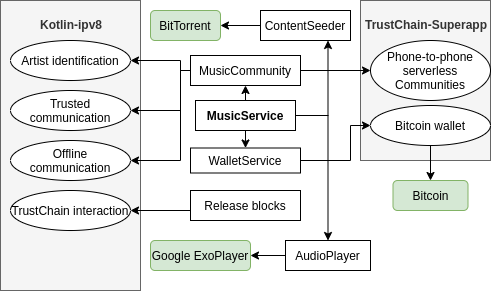
\includegraphics[width=0.6\textwidth]{design/architecture-v1.png}
    \caption{Architecture overview, with in green the external libraries. MusicService is the central component in our system}
    \label{fig:architecture}
\end{figure}

\section{Zero-cost autonomous music industry}
We design a system that takes important first steps towards a zero-cost autonomous music streaming industry, with no intermediaries. In this utopia, intermediaries that add no real value to the industry receive no money. Artists receive near-100\% of all income as they are the core contributors to the industry. Anyone in the community of artists and listeners can create and share music without contacting a party for a contract or allowance. An open protocol over which money and music is exchanged, can be used with different applications, so that users have a choice of user interface. 

Real-world thriving examples such as Linux or Wikipedia are driven by community and effort instead of profit. Consensus is reached through discussion instead of through pyramid schemes. We envision a similar transition for the digital music industry. The next sections will explain the design of our proof-of-concept of MusicDAO, which aims to be the first piece for reaching a fair music industry.

\section{Phone-to-phone censorship-free network}
We design a network which only consists of mobile phones. Every phone cooperates by storing, sharing and validating content. Each mobile phone has access to the same functionalities. The reason for this topology is to have no single, powerful party or centralized server, and that scales naturally. With the latter is meant: the computational power and bandwidth capacity grows with the amount of devices requiring these resources.

A proof-of-concept will show an important step towards mobile infrastructure for the common good: a system in which participants do not lose money and power to greedy intermediaries. Instead, they will benefit from cooperation. This concept aims for absolute fairness, controlled by the community from the ground up instead of dictated top-down. All money going into the system is divided over the participants, following rules written in code that are defined by the community.

\subsection{Censorship-resiliency}
A key attribute of the network is censorship-resiliency. That means that no single authority (company, institution or government) can remove tracks, or prevent devices from participating in the network. Censorship-resiliency is an important requirement for the system because of the issues described in \ref{sec:problem-description-censoring}. Attempting to build a resilient system while using Internet technologies results in a few key challenges as identified by \cite{pouwelse2012censorship} and \cite{di2014bypassing}. To articulate these challenges, we specify a powerful adversary which has the goal to reduce the freedom of a user of the system. The adversary is known to manage the following attacks:
\begin{itemize}
    \item Eavesdropping.
    \item Killing Internet switches. 
    \item Direct censorship: installing malware or spyware.
    \item IP Filtering: block or filter content by restricting access of a specific IP address.
    \item Content filtering: removing or hiding specific content from several hosts.
    \item Confiscating devices: manually take some devices down (a small proportion of the whole network).
\end{itemize}
The following paragraphs explain how MusicDAO is designed to defend against these attacks.

\textit{Eavesdropping}: In a censorship-resistant network, devices talking to each other must trust the network infrastructure to be free of eavesdropping. Preventing eavesdropping can be achieved using end-to-end encryption. However, an adversary may take down certain networking infrastructure to prevent communication altogether (Killing Internet switches).

\textit{Killing Internet switches}: An alternative approach is to establish \textit{direct communication} between devices, which means that data is transmitted device-to-device, without the use of a central access point such such as a router. We use BlueTooth LTE~\citep{townsend2014getting} as a back-up strategy for when Internet traffic is being eavesdropped or when Wi-Fi is killed. This is a widely supported technology in present-day mobile phones and has existing integration into the framework by \cite{mattskala2020}.

\textit{Direct censorship} is another challenge in designing an application. Direct censorship means that there is a piece of code installed on-device that tracks user activity, without the user knowing this. Our solution is two-fold. Firstly, the ecosystem is by default open source. Secondly, the evolution of the code-base is determined by a governance system and majority voting. This means that proposals to change the code-base will need to be voted on by its community. This idea is inspired by previous work from \cite{jentzsch2016decentralized}.

\textit{Content filtering} is not a threat to MusicDAO, because it uses an immutable data structure (see \ref{sec:distributed-storage} for details). This means, in current context, that it is not possible to change or remove any (meta)data of music tracks after they have been published. In addition, multiple copies of track files are available through content duplication. The system uses simple duplication heuristics, such that all objects that a phone receives is stored in cache. This strategy also defends against \textit{confiscating devices} and \textit{IP filtering}. When an adversary takes down, or blocks, a small portion of devices from the network, there will still be back-ups available on the other devices.

\section{Phone-to-phone connectivity}
As mentioned above, MusicDAO is designed to have a network consisting of only mobile phones. Key challenges to establishing and maintaining such a network are: discovering other devices, network connectivity, longevity and scalability.

Every device that wants to participate, will try to find other devices to join the network. Every device also keeps track of a routing table, containing public IP addresses of connected and connectable peers, including latency for each peer. This routing table is inspired by the routing table implemented by BitTorrent DHT~\citep{bittorrentbep5dht}. To discover an \textit{initial} list of devices, we use a bootstrap server, which keeps track of other devices on the network to connect with. A bootstrap server should not be necessary when there are devices on the same Local Area Network that can introduce a new device to the network. However, the network of MusicDAO will be sparse at the start. After a few devices are discovered, the bootstrap server can be disregarded, as new devices are then trivially found via neighbor search.

As there will be no central server, each device acts as both a client and server. As devices may be behind routers or other \textit{Network Address Translators} (NATs), establishing a direct connection between devices is not trivial. To achieve this, we use network address translation (NAT) traversal. NAT traversal is a set of methods used to establish a connection between devices which have no static, public IP address.

To support a healthy evolution of the network, every device will maintain a list of connected devices. Devices will send periodic \textit{keepalive} messages to its connected peers to track which are alive and reachable. By doing this, devices can decide which peers are healthy connections. This list should grow to a few dozen, so that there are always connectable peers.

% NAT traversal
% Identification of devices: IPv8 (move identity section)

% \section{Resiliency and longevity}
% % BlueTooth as backup for Internet kill switches
% % Rigorous duplication of data: one devices leaves the network, data is not lost
% % It is impossible to take down TrustChain data, as proven by Otte et al.
% % In relation to the problems shown with publishing music about for example Tiananmen Square events (see prob desc X), we show the importance of sensor-resiliency at the core of any system that serves the common good.
% % 


% % Our ideas are heavily inspired by previous works by \cite{mattskala2020}

% The network we are designing cannot use central servers or servers from third parties. This network should allow listeners and artists to exchange music and money, without the help from external services. We choose to build a phone-to-phone zero-server network, for the following reasons. Firstly, Mobile phones have the largest share of any type of device using music streaming services. Secondly, if the software that we design and implement runs well on a network consisting of only mobile devices, we can conclude that it will run well on better hardware (such as PCs) as well. 

% We choose to use the Android framework for decentralized apps as proposed by~\cite{mattskala2020}. This gives us a toolbox for building phone-to-phone zero-server apps and make use of its distributed ledger technology to build a public database. It also gives us a public-key infrastructure to identify and authenticate artists. 

\section{Open protocol and artist freedom}
The design of our system contains both an open protocol and an application for the end-user. This is inspired by the ideas from \cite{masnick2019protocols}, who describes that the Internet should go back to open protocols instead of platforms, and that there should be a clear distinction between applications and protocols, so that users have the choice between different applications. Then, every application can have its own strategy of content moderation. This should result in more competition to ``[...] provide better services that minimize the impact of those
with malicious intent, without cutting off their ability to speak entirely''~\citep{masnick2019protocols}.

In our context, we envision different applications using the same streaming, discovery and payment protocol, but with each application having strategies for content filtering and user interfaces. This way, music can not be censored in a centralized manner. Moderation of content happens on the side of the application, so that the user is in control of the settings of moderation and we do not lose freedom of speech or data resiliency.

\section{End-to-end music delivery model}
\label{sec:release-model}
In contrary to the current music publishing situation, dominated by IT gatekeeping and oligarchs as visualized in fig. \ref{fig:current-music-publishing-situation}, we present the desired situation in fig. \ref{fig:desired-music-publishing-situation}. This shows the liberation for artists in publishing their content, and the reduction of single-point-of-failure risks. In this system, artists are free in what they upload. In addition, their content can not be taken down by any authority unless there are no participants in the network. The discovery of content is done using open source, transparent systems and listening data is saved and processed locally.

To achieve this situation, a main component of our system is the storage of metadata and audio files for playlists. We design an abstract model for the structure of this metadata, so that the artist is free in the way to release music content. The artist may publish tracks as part of a single, an EP, an album or any other structured list of tracks, as a Release object.

\begin{figure}
    \centering
    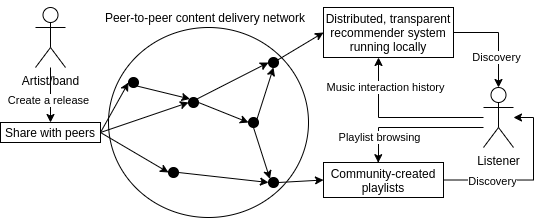
\includegraphics[width=0.8\linewidth]{design/desired-music-publishing-situation.png}
    \caption{Desired music publishing flow using a distributed network}
    \label{fig:desired-music-publishing-situation}
\end{figure}

A Release object contains a list of tracks that are published by a clearly identifiable artist or group of artists. It is modeled as shown in fig. \ref{fig:release-model}. Release objects are shared between peers in the network. By discovering many of those objects, a user can see and browse through them to select a track to play. A Release object merely contains metadata of the tracks. We design the network to have a separate channel for downloading the track files. This is to enable fast discovery and
searching of Releases, as Release objects have a small byte size. 
\begin{figure}
    \minipage{0.2\textwidth}
        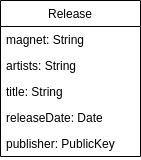
\includegraphics[width=\linewidth]{design/release-model.png}
        \caption{Release blocks structure as seen on TrustChain}
        \label{fig:release-model}
    \endminipage\hfill
    \minipage{0.3\textwidth}
        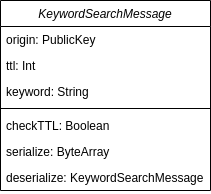
\includegraphics[width=\linewidth]{design/KeywordSearchMessage-model.png}
        \caption{KeywordSearchMessage object sent over IPv8 in MusicCommunity}
        \label{fig:keyword-search-message-model}
    \endminipage\hfill
    \minipage{0.5\textwidth}
    \endminipage
\end{figure}

\section{Identification of participants}
\label{sec:pki-design}
The MusicDAO allows any person to participate, and start publishing or listening to music. It requires a permissionless infrastructure, in which artists can be identified. As we design a system that is fully decentralized, we cannot use a central database to record user identities. Therefore every user generates a unique identity to be used in the network, and must be able to give proof of this identity. We use a public key infrastructure (PKI) which achieve these goals. Every user stores their private and public key on their device, and only share their public key. The keypair has a mathematical property that allows verification of messages that are signed with a private key. By comparing the public key of a peer with their signed message, anyone can verify the authenticity of the message.

In the context of MusicDAO we use this PKI to proof ownership of Release objects. All Release objects are signed using the owner's private key and the signature is added to the object. Any user receiving this object can verify its authenticity.

We choose to use the public key infrastructure as implemented in the TrustChain-Superapp~\citep{mattskala2020}. This abstracts network identifiers such as IP addresses, which may change over time; so it provides a unique identity per Android phone.

\section{Establishing trust and reducing sybil attacks}
In any permissionless infrastructure, legitimacy of parties is not defined by a centralized authority. To still establish trust in the legitimacy of artists, we use the TrustChain DLT~\citep{otte2017trustchain}. Using this technology, we record the history of uploaded tracks in an immutable and transparent way. In essence, every artist adds Release blocks to its personal chain, and due to the interlinking mechanism of TrustChain, it is not possible to hide parts of this history. Every participant can view this timestamped history, as it is public by design. 

This way, an application can inspect the legitimacy of an artist. For example, if an application finds a song X, published by both participant A and B, but the song published by participant A was published later, it can be concluded that A is more trustworthy than B, as B may have copied the song. This system can also be extended trivially to user ratings, or other interactions between parties, to achieve better measurements of trust. This distributed datastore of immutable and transparent histories then becomes a measure against Sybil attacks~\citep{douceur2002sybil} and artist impersonation.

\section{Distributed storage}
\label{sec:distributed-storage}
Central to our system is sharing downloading and storage of audio files and Release objects (see \ref{sec:release-model}). To design a system which has no middlemen or regulators for publishing Releases, and has no central control, a distributed storage system is required. This storage system should have the following properties: immutability (data cannot be tampered with), resiliency (data should be available as long as users want it) and rigorous duplication (all objects should be saved on multiple machines). Distributed ledger technology (DLT) allows for these properties, so we design our system with a DLT as a major component.

One implementation of this technology is TrustChain~\citep{otte2017trustchain} which allows for recording transactions between peers in a linearly scaling public ledger. Every peer has its own immutable and public blockchain which shows its history of transactions with others. This way we can establish trust in a certain party. In our context, we can use this mechanism to estimate trust in artists by inspecting their public history of uploads. We choose TrustChain because of its scalability, its trust mechanism, and because it has a native implementation for Android, as described in \ref{sec:sote-trustchain}. In addition, this implementation allows for offline communication, so users can download and explore new content using Bluetooth or LAN.

\section{Peer-to-peer music sharing}
\label{sec:p2p-music-sharing}
To be able to have low latency for discovering and playing music tracks, while using no central nor high-throughput servers, the network demands participants to upload content continuously. We design the app to, by default, use the network capabilities of the mobile device to upload content as much as possible. This is constrained by networking hardware, data subscription plans and other software running on the phone.

The peer-to-peer file sharing protocol BitTorrent is suitable to share audio files in MusicDAO. We make BitTorrent a design choice as it does not require synchronizing with a global data store, in contrary to IPFS. This means we can build a metadata store independently from BitTorrent (for example, using TrustChain as explained in \ref{sec:distributed-storage}). BitTorrent also has stable implementations for Android.

\section{Distributed search}
For searching content we use introduce our simple distributed algorithm. Pseudocode of this algorithm is shown in alg. \ref{alg:algorithm-distributed-search}. It asks peers around for content tagged with some keyword. When a peer finds a match on their local database, it sends this Release object to the original asking peer. Otherwise it forwards the query to their neighbours, after reducing the time-to-live property by 1. The messages stop being forwarded once their time-to-live property hits below 1. The structure of search messages are shown in fig. \ref{fig:keyword-search-message-model}. 

This algorithm is inspired by the more general Gnutella search and retrieval protocol~\citep{kronfol2002fasd}. Gnutella is widely used and has over a million users.

\begin{algorithm}
\caption{Distributed algorithm for remote search}
\begin{algorithmic}
\Function{DistributedSearch}{$query, ttl, maxPeers, minResults$}\Comment{Device initiates the search}
    \State $results\gets localSearch(query)$\Comment{Filter local database}
    \If {$|results|\leq minResults$}
        \State $origin \gets myAddress()$\Comment{Address of the device initiating the search}
        \For{$i\gets 1, maxPeers$}
            \State $peer \gets peers[i]$\Comment{Select a random neighbor}
            \State $sendQuery(origin, peer, query, ttl)$
        \EndFor
    \Else
        \State \textbf{return} $results$
    \EndIf
\EndFunction
\Function{OnQuery}{$origin, peer, query, ttl$}\Comment{This is called when a query is received}
    \If $ttl\leq 0$
        \State \textbf{return}
    \EndIf
    \State $ttl \gets ttl-1$
    \State $results\gets localSearch(query)$
    \If {$|results|\le 1$}
      \For{$i\gets 1, maxPeers$}
            \State $peer \gets peers[i]$
            \State $sendQuery(origin, peer, query, ttl)$
        \EndFor
    \Else
        \State $sendResults(origin, results)$\Comment{Send the results back directly to the origin}
    \EndIf
\EndFunction
\end{algorithmic}
\end{algorithm}

\begin{figure}
    \centering
    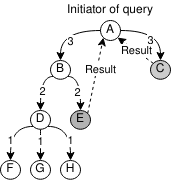
\includegraphics[width=0.4\textwidth]{design/search-algorithm-diagram.png}
    \caption{Search algorithm execution example: node A initiates a search query.}
    \label{fig:search-algorithm-diagram}
\end{figure}

Fig. \ref{fig:search-algorithm-diagram} shows a visualization of execution of the algorithm in a small network. Participant A wishes to find a set of results $R$ for query $q$, so it initiates a search query. Firstly it inspects its local database. Because there are $|R|=0$ results, it sends a query to its neighboring peers (B and C). The peers depicted in grey finds $|R|\gte 1$ results; they send their result back directly to A and do no other action. Other peers forward $q$ to its neighbors, reducing $q_{ttl}$ by 1. \textit{Time-to-live} hits 1 when arriving in F,G,H so the search terminates. 

\section{Transparent money flow}
Figures \ref{fig:current-money-flow} and \ref{fig:desired-money-flow} visualize, in a simplified fashion, the difference of how money flows in the current situation and in MusicDAO. It shows that, when intermediaries are cut from the flow, artists will have a higher income for the same fees from the listener. Streaming services and record holders introduce many overhead costs. Our system allows artists to publish their songs without the need to contact a label. The biggest difference in income will be seen for independent artists, as streaming services gives particularly low payouts for unsigned artists.

As we are designing a system with no intermediaries, it should be possible to give money directly to artists. Cryptocurrency allows for peer-to-peer payments which achieve this goal, so we use this in the MusicDAO. Cryptocurrency payments will be used for two different functionalities: a user can send a donation to an artist, or a user can pay artists using a monthly subscription system. This subscription system pays artists that the user listened to, using the Artist Income Division Algorithm (see \ref{sec:aida-design}). 

In the desired money flow, we have a  Fig. \ref{fig:desired-money-flow} shows another component: an automated and transparent payment division system. In practice, this should be an algorithm running locally on the machine of the user which calculates how much money should go to each of the shareholders of a particular song. Currently, record holders have this task, but there exists no transparent system for this, so they can give low payouts to its artists. We design the transparent payment system to be an immutable record on a distributed ledger, on which a specification of the exact shares per artists are written down. This can be implemented using TrustChain blocks~\citep{otte2017trustchain}.

We choose to use Bitcoin as a cryptocurrency as it has shown to be a fully peer-to-peer, secure and popular payment system, and it does not rely on any third parties to run. It also allows for making a experimentation environment without any high-throughput external servers. 

\begin{figure}
    \minipage{0.6\textwidth}
        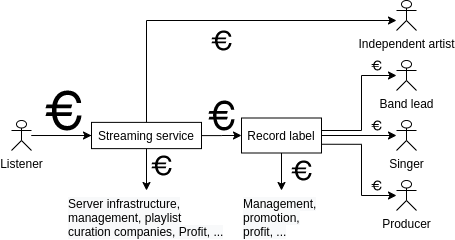
\includegraphics[width=\linewidth]{design/current-money-flow.png}
        \caption{Money flow: current situation (simplified)}
        \label{fig:current-money-flow}
    \endminipage\hfill
    \minipage{0.4\textwidth}
        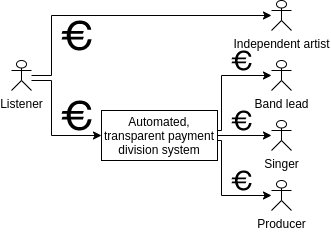
\includegraphics[width=\linewidth]{design/desired-money-flow.png}
        \caption{Money flow: desired situation}
        \label{fig:desired-money-flow}
    \endminipage
\end{figure}
\subsection{Wallet}
Cryptocurrency implementations allow for private/public key-pairs which can be interpreted as a kind of wallet; the funds can only be unlocked by a holder of the private key. In the case of MusicDAO we design the app to include a wallet for every user. To receive money, every artist should share their public key to all of their listeners. To achieve this, the public key of their cryptocurrency wallet is included as a property of the Release objects (see \ref{sec:release-model}). As there are no institutions or banks involved in storing money, users will be required to keep their private key safe.

\subsection{Artist Income Division Algorithm}
\label{sec:aida-design}
To provide a stable income for artists, in the form of reoccurring payments, we design the Artist Income Division Algorithm. This algorithm calculates how subscription money is split into payments to artists. The user can enable a periodic payment. This money is then divided over the artists the user listens to, in proportion to the amount of interaction with each artist. Interaction can be measured in e.g. time listened, plays or feedback in the form of likes. The details of this division is explained in the implementation section of AIDA (see TODO).

\section{Content popularity gossip protocol}

\section{Scalability}
MusicDAO is scalable by using a scalable accounting system (see \ref{sec:distributed-storage}) and distributed file system (see \ref{sec:p2p-music-sharing}). Every device records its own history. When a device wants to publish music, it only transacts with one other party, to sign the metadata record. As such, there is no global consensus, nor a global ordering of transactions, so all records are processed in parallel.

In addition, by using BitTorrent as the streaming/content layer, any participant can publish a torrent with music, without needing to interact with any other peer. 

Finally, the transaction system, Bitcoin, may become a bottleneck in scalability. It requires global consensus and a voting process for every transaction. However, as of the time of writing, there is no mature and more scalable alternative as peer-to-peer payment system technology. We do not consider centralized technologies as that would concentrate power, in contrary to the aim of this thesis.